% ! TeX root = ../thesis-main.tex
%----------------------------------------------------------------------------------------
\chapter{Implementation}
\label{chap:implementation}
%----------------------------------------------------------------------------------------

This chapter documents the implementation details of the models and libraries designed, as well as additional tools and extensions developed as research experiments and proof of concepts.
%
The implementation of the \texttt{core} and \texttt{simulator} modules has no external, third-party dependencies apart from the Scala standard library, thus satisfying the requirement \textit{T.7} from \cref{chap:analysis->sec:requirement-analysis}.
%
In particular, the chapter covers the implementation of an experimental \texttt{FoldhoodLibrary}, that demonstrates the expressiveness of the \this design by implementing an \ac{API} for \texttt{foldhood} and \texttt{foldhoodPlus} similar to the original ScaFi, and the prototype of a different implementation of the \texttt{AggregateFoundation} trait, which adds compile time assertions on the user code to prevent common mistakes and improve the quality of aggregate programs, at the expense of more complicated signatures of library methods, following requirement \textit{F.8} from \cref{chap:analysis->sec:requirement-analysis}.
%
The chapter also covers the integration of \this with the Alchemist simulator (requirement \textit{F.4} from \cref{chap:analysis->sec:requirement-analysis}), which enables graphical and more realistic simulations, as well as additional proof of the functionality of \this.

\section{Implementation of the XC operational semantics} \label{chap:implementation->sec:xc-ops}

The implementation of the operational semantics as described in paper\cite{xc} follows the design of \cref{chap:design->sec:final-dsl->subsec:exchange-calculus-semantics-design} by defining a concrete class that inherits from \texttt{ExchangeCalculusSemantics}.
%
Given that the same class serves as context for the execution of aggregate programs' rounds, following the engine design of \cref{chap:design->sec:final-dsl->subsec:engine}, it implements the \texttt{Context} interface too.

The implementation is named \texttt{BasicExchangeCalculusContext}, because it is meant to provide a simple yet readable and reliable implementation, without pursuing premature optimizations or additional features.
%
A more advanced implementation could be developed in the future, maybe specifically tailored to some destination platform or network implementation.
%
In order to maximize the reusability of its code, the logic and behavior that compose the operational semantics has been broken down into several mixin layers, with their dependencies declared through self-type annotations and abstract members.
%
These mixin layers have been organized into two packages based on their reusability: \texttt{context.common} with the most general and reusable mixins, and \texttt{context.exchange} with the mixins that are specific to the exchange calculus, as shown in \cref{fig:context-mixins-common,fig:context-mixins-exchange}.

\begin{figure}
    \centering
    \caption{Exchange Calculus context mixins: \ac{UML} diagram of the mixin layers in package \texttt{common}, stripped of transitive dependencies.}
    \label{fig:context-mixins-common}
    \bigskip
    \resizebox{\linewidth}{!}{
        \input{diagrams/context-mixins/Context Mixins - Common.latex}
    }
\end{figure}

\begin{figure}
    \centering
    \caption{Exchange Calculus context mixins: \ac{UML} diagram of the mixin layers in package \texttt{exchange}, stripped of transitive dependencies.}
    \label{fig:context-mixins-exchange}
    \bigskip
    \resizebox{\linewidth}{!}{
        \input{diagrams/context-mixins/Context Mixins - Exchange.latex}
    }
\end{figure}


\subsection{The stack-based semantics implementation}

Without using Scala 3 macros everywhere an aggregate expression is written, the \ac{AST} of an aggregate program is not directly available to the semantics implementation.
%
Consequently, the semantics implementation has to track the invocation of its primitives into an explicit stack-like \ac{ADT}, while building the \texttt{Export} value tree using the paths traced by the stack.
%
If a primitive invocation is nested inside another, the invocation trace is pushed into the stack, and the nested expression is evaluated, potentially growing the stack but leaving it unchanged at the end of the evaluation, and then the trace is popped from the stack.
%
This logic is implemented in the \texttt{scope} method of \texttt{StackSemantics} and is employed by the \texttt{xc} implementation of \texttt{exchange.ConstructsSemantics}.
%
For instance, the program in \cref{lst:value-tree-example}, at the first execution round with the \texttt{BasicExchangeCalculusContext}, would produce the value tree in \cref{fig:value-tree-example}.

\lstinputlisting[float, language=Scala, caption={Example of aggregate program that produces the value tree in \cref{fig:value-tree-example}.}, label={lst:value-tree-example}]{listings/value-tree-program.scala}

\begin{figure}
    \centering
    \caption{Example of value tree produced by the program in \cref{lst:value-tree-example}.}
    \label{fig:value-tree-example}
    \bigskip
    \resizebox{0.5\linewidth}{!}{
        \input{diagrams/value-tree/Value Tree Example.latex}
    }
\end{figure}

Alignment is implemented by comparing the current stack with the neighbor's value trees: if a path prefix is in common, the device is aligned with the given neighbor.
%
In order to distinguish \texttt{exchange} invocations that are not part of the same conditional branch, it is necessary that the \texttt{branch} construct is invoked in place of Scala's \texttt{if}, and that the \texttt{branch} construct is implemented to push a branch identifier into the stack using the scope method, thus misaligning devices who took different branches.
%
A known limitation and pitfall of this solution, besides making programmers understand the need to use \texttt{branch} instead of \texttt{if}, is boolean short-circuiting, which behaves similarly to the \texttt{if} construct, in the sense that it can happen to skip the evaluation of some exchange calls without tracing the conditional branch in the stack.
%
When that happens, the resulting behavior is unpredictable and will probably lead to runtime errors.

\texttt{InboundMessagesSemantics} is responsible for providing the set of currently aligned devices as well as retrieving the values corresponding to the current traced path from their value trees.
%
\texttt{OutboundMessagesSemantics} is responsible for building the export value tree using the current path and the values passed to the \texttt{sendMessages} method.
%
Once the program round has completed, and the \texttt{Engine} asks for the \texttt{Export} value tree, the sent messages are reorganized into a different value tree for every known neighbor, plus the current device, because memory is modeled as a self-message, and a default value tree for every new neighbor that appears during sleep time.
%
This is the reason why the \texttt{Export} is an alias for a \texttt{MapWithDefault} while the \texttt{Import} is an alias for a \texttt{Map}, with both \ac{ADT} immutable.

Inside a value tree, values of different types are stored together under a common type, and they need to be converted back to their original types when extracted from the tree.
%
For this reason, \texttt{MessageSemantics} offers two methods, \texttt{open} and \texttt{close}, responsible for the conversion from and to the common type, defined with an abstract type member called \texttt{Envelope}.
%
In a real-world distributed system, an \texttt{Envelope} could be a sequence of bytes, containing the serialized stream from shared objects.
%
For the scope of \this, all the simulations are executed using the \texttt{MessageSemantics.Basic} implementation, which simply casts the values to and from \texttt{Any}, which works because the simulations are run in a single JVM, and the \texttt{Any} type is the root of the Scala type hierarchy.

\section{The build system}

Following the requirements listed in \cref{chap:analysis->sec:requirement-analysis}, the chosen build system for the project is \ac{SBT}, in particular version \texttt{1.9.8}, following requirement \textit{T.3} from \cref{chap:analysis->sec:requirement-analysis}.
%
The build tool has been customized with the following plugins:
\begin{itemize}
    \item \texttt{sbt-scalafix} to lint the code with \textit{scalafix}, further explained in \cref{chap:evaluation->sec:code-style}, following requirement \textit{T.6} from \cref{chap:analysis->sec:requirement-analysis};
    \item \texttt{sbt-scalafmt} to lint the code with \textit{scalafmt}, further explained in \cref{chap:evaluation->sec:code-style}, following requirement \textit{T.6} from \cref{chap:analysis->sec:requirement-analysis};
    \item \texttt{sbt-scalajs} and \texttt{bt-scalajs-crossproject} to cross-build the project for \textit{JavaScript} with \textit{scala-js}, following requirement \textit{T.4} from \cref{chap:analysis->sec:requirement-analysis};
    \item \texttt{sbt-scala-native} and \texttt{sbt-scala-native-crossproject} to cross-build the project for \textit{native} with \textit{scala-native}, following requirement \textit{T.5} from \cref{chap:analysis->sec:requirement-analysis}.
\end{itemize}
%
In addition to that, the Dotty compiler has been customized with flags that enhance the quality of the code, such as the aforementioned \textit{explicit nulls} and \textit{multiversal equality}, but also enforcement for indentation over curly braces style, warnings as errors, safe initialization checks, warnings on value discards, and more (requirement \textit{T.2} from \cref{chap:analysis->sec:requirement-analysis}).

\section{The \quotes{FoldhoodLibrary}} \label{chap:implementation->sec:foldhood-library}

As a proof of concept of the expressiveness of the \this design, an experimental library has been developed, called \texttt{FoldhoodLibrary}, which provides an \ac{API} for the \texttt{foldhood} and \texttt{foldhoodPlus} constructs as defined in the original ScaFi library, representing in a way an internal \ac{DSL} written in terms of another.
%
The library works for any aggregate context that supports the \texttt{FieldCalculusSyntax}, and implements \texttt{foldhood}, \texttt{foldhoodPlus}, \texttt{nbr}, and \texttt{nbrRange} for contexts that also support \texttt{DistanceSensor}.
%
The resulting \ac{API} can be seen used in \cref{lst:foldhood-library-usage},
where \texttt{nbr} is not the same as the one defined in \texttt{FielCalculusLibrary} but has a different signature, that takes a lazy expression of type \texttt{=> T} and returns a \texttt{T}.
%
When evaluating a foldhood, the expression is evaluated as is and the values passed to \texttt{nbr} are recorded and returned in order, then shared with neighbors.
%
Then, for each aligned neighbor, the same expression is re-evaluated, this time substituting the \texttt{nbr} return values with the ones coming from neighbors, in the right order to match the expression.
%
If the context implements the \texttt{DistanceSensor} trait, \texttt{nbrRange} can be invoked to return the distance from the current node to the neighbor evaluated in the foldhood.
%
The only difference between \texttt{foldhood} and \texttt{foldhoodPlus} is that the former does not include the expression value of the current node in the folding result, while the latter does.
%
The example of \cref{lst:foldhood-library-usage} demonstrates that \texttt{nbr} can be used with arguments of any type, as long as they type check in the foldhood expression.

\lstinputlisting[float, language=Scala, caption={Usage example of the \texttt{FoldhoodLibrary}.}, label={lst:foldhood-library-usage}]{listings/foldhood-usage.scala}


\section{Context-based constraints on shared values} \label{chap:implementation->sec:context-based-constraints}

This proof of concept has been implemented on a different feature branch of the repository, as it represents a very impactful change on the entire framework.
%
The idea is to use context bounds on every method that is supposed to share values with neighbors or self, such as \texttt{exchange}, \texttt{nbr}, \texttt{share}, \texttt{distanceTo}, and so on.
%
Through these context bounds, the types able to be shared can be restricted by a set of rules, that, if not satisfied, won't provide the context parameter needed to invoke the method.
%
The type class used as bound is called \texttt{Shareable}, and its counterpart negating it is named \texttt{NotShareable}, as shown in \cref{lst:shareable-type-classes}.
%
By default, in order to allow libraries that abstract over the semantics implementation to share at the very least primitive types and classes marked as \texttt{Serializable}, a global given instance of \texttt{Shareable} is provided for subtypes of \texttt{AnyVal} or \texttt{Serializable}.
%
Given that the \texttt{Shareable} type class is marked as \texttt{open} and has a public constructor, semantics and their implementations can extend the set of types that satisfy the constraints, by providing additional given instances of the type class, and optionally adding ad-hoc behavior to the type class with extensions.
%
As a side-effect, the \texttt{Shareable} could potentially be instantiated manually to force any type to be shareable, probably resulting in a runtime error during the actual serialization phase that would have occurred anyway without this whole feature enabled.
%
Nevertheless, in a typical scenario, the constraint works as expected, as shown in \cref{lst:shareable-type-classes-usage}, where the \texttt{Shareable} constraint is violated by the attempt to share a value of type \texttt{AggregateValue[Int]}, while it is marked as \texttt{NotShareable} by the \texttt{AggregateFoundation}.
%
In the same snipped, the new signature of the \texttt{nbr} method with the context bound shows how signatures get affected by this change, in case it was merged and applied to the main branch.

\lstinputlisting[float, language=Scala, caption={Definition of the \texttt{Shareable} and \texttt{NotShareable} type classes.}, label={lst:shareable-type-classes}]{listings/context-based-constraints-definition.scala}

\lstinputlisting[float, language=Scala, caption={Usage example of the \texttt{Shareable} type class, that demonstrates a violation of the constraint.}, label={lst:shareable-type-classes-usage}]{listings/context-based-constraints-violation.scala}


\section{Integration with the Alchemist simulator}

As stated in the GitHub repo\footnote{\url{https://github.com/AlchemistSimulator/Alchemist}}, Alchemist is a simulator for pervasive, aggregate, and nature-inspired computing.
%
Originally, Alchemist was conceived as a chemical-oriented multi-compartment stochastic simulation engine, generic enough that could be adapted to simulate a wide range of systems, even if unrelated to the chemistry domain\cite{alchemist}.
%
The integration with Alchemist enables a whole new simulation experience, thanks to the graphical interface and the ability to simulate most of the relevant properties of real-world \ac{CAS}.
%
Integrating with the simulator consists, in practice, of implementing an \textit{incarnation}, which is a set of classes that bridge the Alchemist models of molecule, reactions, and concentration with the desired models of the simulation.
%
Inside an Alchemist simulation of a network of devices, each device is represented as a \texttt{Node}, and the incarnation implementation adds to each node an implementation of a \texttt{Network}, an engine instance, and a reference to the aggregate program to simulate.
%
Each node has visibility over its neighbors and takes care to send outbound messages to the right recipients when invoked, after the execution round.
%
During each of the rounds, the engine will invoke the aggregate program using \textit{Java reflections}, because the program's fully qualified name is passed as a string through the configuration file written in \textit{yaml}, such as the one in \cref{lst:alchemist-demo-configuration}.
%
If the provided configuration is run with the program of \cref{lst:alchemist-demo-program}, the expected output will be similar to the snapshot of \cref{fig:alchemist-simulation}.

\lstinputlisting[float, style=yaml, caption={Example of Alchemist configuration file.}, label={lst:alchemist-demo-configuration}]{listings/alchemist-demo.yml}

\lstinputlisting[float, language=Scala, caption={Example of aggregate program that can be run with the Alchemist simulator.}, label={lst:alchemist-demo-program}]{listings/alchemist-demo.scala}

\begin{figure}
    \centering
    \caption{Snapshot of the Alchemist simulation of the program in \cref{lst:alchemist-demo-program}, with the configuration in \cref{lst:alchemist-demo-configuration}.}
    \label{fig:alchemist-simulation}
    \bigskip
    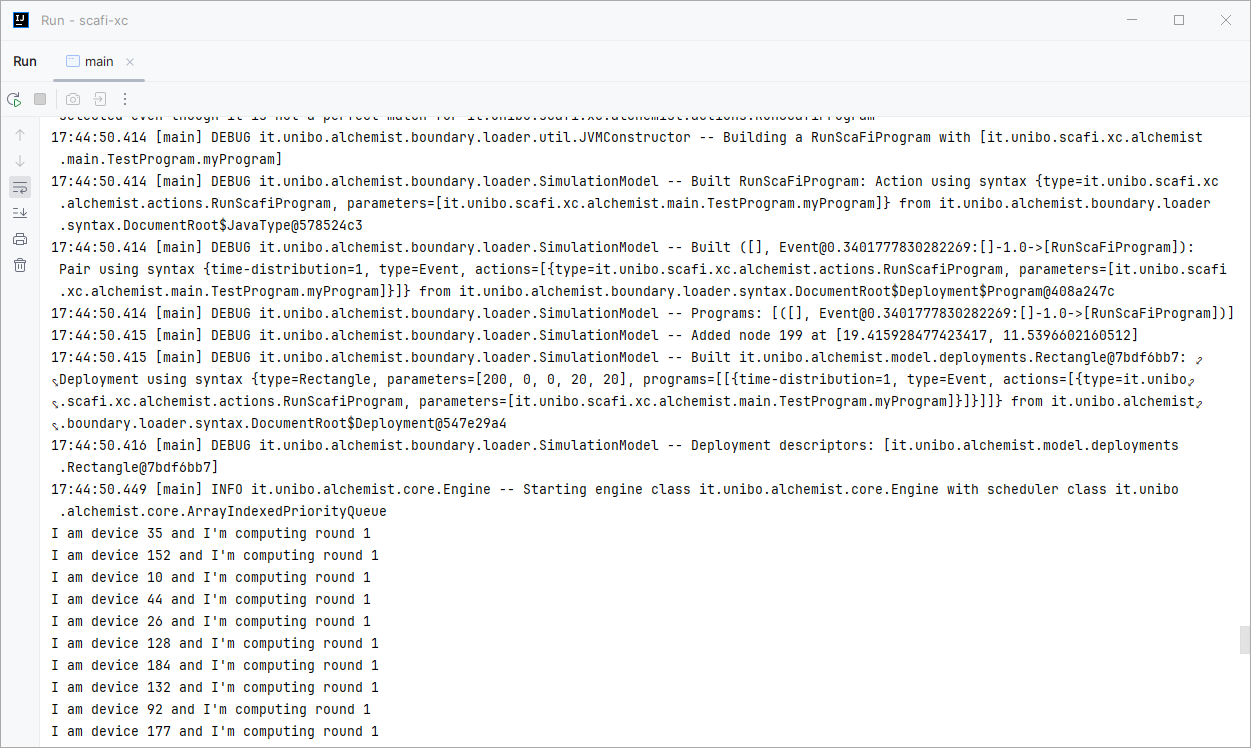
\includegraphics[width=\linewidth]{figures/alchemist-demo.png}
\end{figure}
